\documentclass[11pt]{article}
\usepackage[a4paper,margin= 2cm]{geometry}
\usepackage{graphicx}
\usepackage{caption}
\usepackage{subcaption}

\title{\LARGE{\bf{Task 5 - QR Decomposition and Least Squares }}}
\author{\Large{\bf{Kirtan Patel - AE19B038}}}
\date{}

\begin{document}

\maketitle 

\section{Introduction}
Often times the data that we get is not linear and using higher order polynomials gives a better fit than using Linear Regression.\\

In Task 2,  we performed Linear Regression on each dataset, taking the first 50,100 and 200 datapoints one after the other.

Plotting the Regression line as 
\[Y = \beta_1 X + \beta_0\]
we record the values obtained for $\beta_0$ and $\beta_1$.\\

We did that by converting it into matrix form as : 
\[A.x = B\] 
where x = [$\beta_0~~\beta_1$]\textsuperscript{T}. We further solved this by premultiplying A$^T$, getting a square matrix on the LHS (A$^T$.A gives a square matrix) and then finding the inverse of this square matrix. We pre-mulitply the inverse matrix and get the solution for vector x, ans in-turn get the coefficients of Linear Regression.\\

Finding the inverse of a matrix is computationally heavy and hence there are other optimized methods (eg. LU Decomposition) which help us reduce the complexity of the code. One such method is the QR decomposition of matrix A.

\section{QR Decomposition}
The QR decomposition (also called the QR factorization) of a matrix is a decomposition
of the matrix into an orthogonal matrix and a triangular matrix. A QR decomposition of
a real square matrix A is a decomposition of A as:
\[A = QR\]
where Q is an orthogonal matrix (i.e. Q$^T$Q = I) and R is an upper triangular matrix. If A is nonsingular, then this factorization is unique.\\

There are several methods for actually computing the QR decomposition. One of such
method is the Gram-Schmidt process.\\

After seperating A into Q and R, we pre-multiply Q$^T$ and since Q is orthogonal, we get : 
\[ R.x = Q^T B\]

And since R is an upper triangular matrix, we can solve for the components of x using back substitution form the last term to the first term (bottom to the up). This process is computationally faster than finding the inverse of a matrix and hence is used. There are other faster processes as well which are computationally more efficient than the processes mentioned and discussed here.
\newpage
\subsection{Gram-Schmidt Process}
\begin{figure}[h!]
	\centering
	\centering
	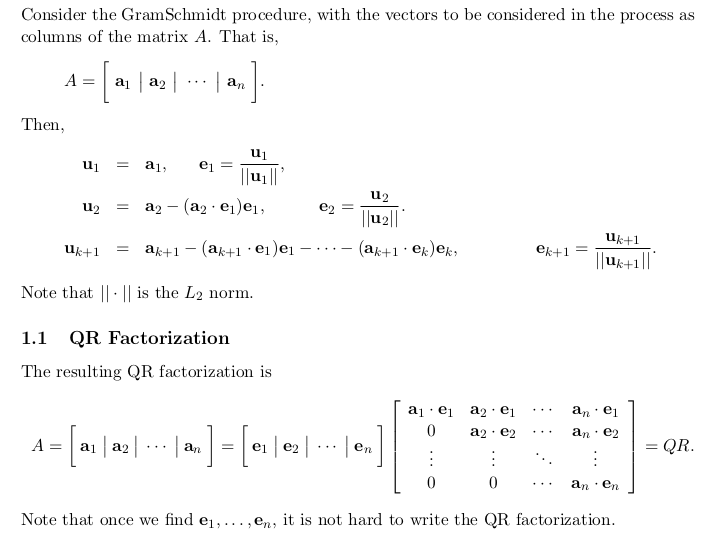
\includegraphics[width=\linewidth]{GS_Process}
	\label{GS_orthogonalization}
\end{figure}

\section{Task 5}
Keeping the above mentioned points in mind, in Task 5, we are given a data set. Using QR Decomposition with Gram-Schmidt Orthogonalization and back-substitution(without using canned routines), we need to find the Regression Coefficients for a quadratic regression. i.e. 
\[ Y = \beta_2 x^2 ~+~ \beta_1 x ~+~ \beta_0\]

Furthermore, we have to compare this method of solving the Matrix Equation to the method of matrix inversion used in Task 2. The comparison is to be made on the  accuracy and the time taken for the methods to execute and return the coefficients.\\

We were even asked to justify if the bi-quadratic regression line is a better fit.
\[Y = \beta_4 x^4 ~+~ \beta_3 x^3 ~+~\beta_2 x^2 ~+~ \beta_1 x ~+~ \beta_0\]

To take measurement for the time parameter, the built-in time module has been imported, whereas to measure the accuracy/fit of the model, instead of simple square-error, the R-sqaure is used. R-squared evaluates the scatter of the data points around the fitted regression line. It is also called the coefficient of determination, or the coefficient of multiple determination for multiple regression. For the same data set, higher R-squared values represent smaller differences between the observed data and the fitted value. Usually, the larger the R2, the better the regression model fits your observations. 

\section{Results}
\begin{figure}[h!]
	\centering
	\centering
	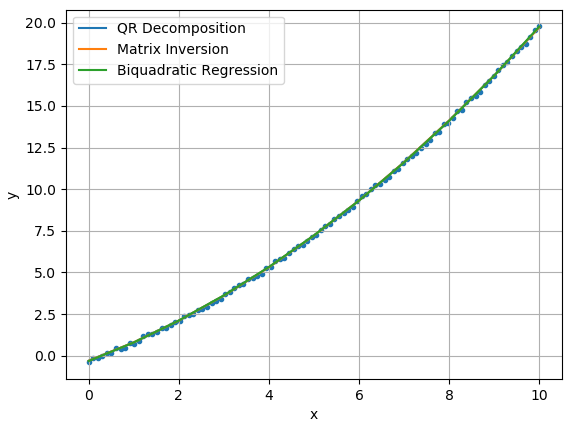
\includegraphics[width=0.7\linewidth]{Task5}
	\label{Plot}
\end{figure}

As we can see the plot is highly intervined, and the regression lines from all the methods are extremely similar.

\subsection{Regression Coefficients}
Tabulating the results obtained for the Regression Coefficients.
\begin{table} [h!]
	\centering
	\begin{tabular}{| l | l | l | l | l | l |}
		\hline
		Model - Solving Method & $\beta_0$ & $\beta_1$ & $\beta_2$  & $\beta_3$ & $\beta_4$\\
		\hline \hline
		Quadratic Model - QR Decomposition & -0.30539967 & 1.00663479 & 1.0066348  & na & na \\
		\hline 
		Quadratic Model - Matrix Inversion & -0.30539967 & 1.00663479  & 0.0996548  & na & na \\
		\hline 
		Biquadratic Model - QR Decomposition & -0.31756812 & 1.00848424  & 0.1056871  & -0.0017 & 0.00011314\\
		\hline
	\end{tabular}
\end{table}

\subsection{Time Taken}
The computational times were not coming out to be constant but were varying around a range. Thus a range of runtimes has been tabulated.
\begin{table} [h!]
	\centering
	\begin{tabular}{| l | l |}
		\hline
		Model - Solving Method & time (ms)\\
		\hline \hline
		Quadratic Model - QR Decomposition & 0.30~-~0.35 \\
		\hline 
		Quadratic Model - Matrix Inversion & 0.40~-~0.50 \\
		\hline 
	\end{tabular}
\end{table}

\subsection{Accuracy}
\begin{table} [h!]
	\centering
	\begin{tabular}{| l | l |}
		\hline
		Model - Solving Method & R-squared\\
		\hline \hline
		Quadratic Model - QR Decomposition & 0.9998552213770414 \\
		\hline 
		Quadratic Model - Matrix Inversion & 0.9998552213770575 \\
		\hline 
		Biquadratic Model - QR Decomposition & 0.9998596029906132 \\
		\hline 
	\end{tabular}
\end{table}
We can see that while both the Quadratic Models have almost same accuracy, the Biquadratic Model is slightly more accurate.
\pagebreak 

\section{References}
\begin{enumerate}
	\item https://www.math.ucla.edu/~yanovsky/Teaching/Math151B/handouts/GramSchmidt.pdf
	\item
	https://www.r-bloggers.com/2017/03/qr-decomposition-with-the-gram-schmidt-algorithm/
	\item
	https://en.wikipedia.org/wiki/Gram$\%$E2$\%$80$\%$93Schmidt$\_$process
	\item
	http://math.iit.edu/~fass/477577$\_$Chapter$\_$4.pdf
	\item
	https://www.youtube.com/watch?v=w2FKXOa0HGA
\end{enumerate}




\end{document}